\documentclass[pageno]{jpaper}


\usepackage{graphicx}
\usepackage{subfig}
%Removing the geometry package used for Tighter Format
%\usepackage{geometry}
%\usepackage{times}
\usepackage{textcomp}
\usepackage{multirow}
\usepackage{framed}
\usepackage{amsmath}
\usepackage{listings}
\usepackage{hyperref}
\usepackage{enumitem}
\usepackage{amssymb}

% \newcommand{\submissionnumber}{144}
% \newcommand{\sysname}{Il\'uvatar}
\newcommand{\D}{\emph{D}}
\newcommand{\Dmax}{\emph{D\_max}}
\newcommand{\T}{\emph{T}}
\newcommand{\VT}{\emph{VT}}
\newcommand{\GlobVT}{\emph{Global\_VT}}
\newcommand{\FinVT}{\todo{REMOVE: finish\_vt}}
% \newcommand{\QName}{MQ-FLQ}
% \newcommand{\QNameFull}{Multi-Queue Fair \& Local Queuing}
\newcommand{\QName}{MQFQ-Sticky}
\newcommand{\QNameFull}{\QName}
\newcommand{\batch}{\texttt{Batch}}
\newcommand{\naive}{\texttt{FCFS Naïve}}
\newcommand{\fcfs}{\texttt{FCFS}}

% \usepackage{tikz}

% \RequirePackage[normalem]{ulem}
% \RequirePackage{color}\definecolor{RED}{rgb}{1,0,0}\definecolor{BLUE}{rgb}{0,0,1}
\providecommand{\DIFadd}[1]{{\protect\color{blue}\uwave{#1}}}
\providecommand{\DIFdel}[1]{{\protect\color{red}\sout{#1}}}
%DIF SAFE PREAMBLE
\providecommand{\DIFaddbegin}{}
\providecommand{\DIFaddend}{}
\providecommand{\DIFdelbegin}{}
\providecommand{\DIFdelend}{}
%DIF FLOATSAFE PREAMBLE
\providecommand{\DIFaddFL}[1]{\DIFadd{#1}}
\providecommand{\DIFdelFL}[1]{\DIFdel{#1}}
\providecommand{\DIFaddbeginFL}{}
\providecommand{\DIFaddendFL}{}
\providecommand{\DIFdelbeginFL}{}
\providecommand{\DIFdelendFL}{}
%DIF END PREAMBLE EXTENSION ADDED BY LATEXDIFF

\def\Section {\S}

\newcommand{\squishlist}{
 \begin{list}{$\bullet$}
  { \setlength{\itemsep}{0pt}
     \setlength{\parsep}{3pt}
     \setlength{\topsep}{3pt}
     \setlength{\partopsep}{0pt}
     \setlength{\leftmargin}{1.5em}
     \setlength{\labelwidth}{1em}
     \setlength{\labelsep}{0.5em} } }
	
\newcommand{\squishlisttwo}{
 \begin{list}{$\bullet$}
  { \setlength{\itemsep}{0pt}
     \setlength{\parsep}{0pt}
    \setlength{\topsep}{0pt}
    \setlength{\partopsep}{0pt}
    \setlength{\leftmargin}{2em}
    \setlength{\labelwidth}{1.5em}
    \setlength{\labelsep}{0.5em} } }

\newcommand{\squishend}{
  \end{list}  }

% \newcommand{\squishenum}{
%   \begin{enumerate}{$\bullet$}
%     { \setlength{\itemsep}{0pt}
%       \setlength{\parsep}{0pt}
%       \setlength{\topsep}{0pt}
%       \setlength{\partopsep}{0pt}
%       \setlength{\leftmargin}{2em}
%       \setlength{\labelwidth}{1.5em}
%       \setlength{\labelsep}{0.5em} } }
  
% \newcommand{\squishenumend}{
%   \end{enumerate}  }

\newcommand{\alert}[1] {\textcolor{red} {\textsc{#1}}}

\newcommand{\myfbox}[1] {\noindent \fbox{\parbox{0.5\textwidth} {#1}}}

\newcommand{\mhead}[1] {\noindent \textbf{#1.}}

\newcommand*\mean[1]{\overline{#1}}

\newcommand{\eat}[1]{}

\newcommand{\compresslist}{%
  \setlength{\itemsep}{1pt}%
  \setlength{\leftmargin}{1.5em}
  \setlength{\labelwidth}{1em}
  \setlength{\parskip}{0pt}%
  \setlength{\parsep}{0pt}%
%  \setlength{\itemindent}{-10pt}%
}

\newcommand{\myfigspace}[0]{-0.3cm}
\newcommand{\bigfigspace}[0]{-0.9cm}
\newcommand{\captionspace}[0]{-0.25cm}
\newcommand{\subsecspace}[0]{-0.1cm}
\newcommand{\largesubsecspace}[0]{-0.38cm}

\newcommand\prat[1]{\textcolor{red}{(Prateek: #1)}}

\newcommand{\quotes}[1]{``#1''}
\newcommand{\todo}[1]{\textcolor{orange}{TODO: #1}}
\newcommand{\alex}[1]{\textcolor{blue}{Alex: #1}}
% https://tex.stackexchange.com/a/7045
\newcommand*\circled[1]{\tikz[baseline=(char.base)]{
            \node[shape=circle,draw,inner sep=2pt] (char) {#1};}}


\newcommand{\funcname}[1]{\texttt{#1}}

\newcommand{\asplossubmissionnumber}{1225}

\usepackage[normalem]{ulem}


\begin{document}
%-------------------------------------------------------------------------------

\title{FaasCache: Keeping Serverless Computing Alive With Greedy-Dual Caching \\
Extended Abstract}

%don't want date printed
\date{}

% make title bold and 14 pt font (Latex default is non-bold, 16 pt)
\author{}

\maketitle 

\thispagestyle{empty}

\section{Motivation: Keep-alive in FaaS}
\vspace*{\subsecspace}
% Bit too long.... 
Functions as a Service (FaaS) is an emerging and popular cloud computing model, where applications use cloud resources through user defined ``functions'' that execute application code~\cite{jonas_cloud_2019}.
%By handling all aspects of function execution, including resource allocation, cloud platforms can thus provide a ``serverless'' computing model where users do not have to explicitly provision and manage cloud resources (i.e., virtualized servers).
%
FaaS is being used by different applications such as web services, API services, parallel and scientific computing, and in machine learning pipelines. 
%
The execution time of each function is typically short---in the range of a few milliseconds to a few seconds. 


While Functions as a Service (also called serverless computing) promises to revolutionize how applications use cloud resources, the tight latency requirement and the wide diversity in function characteristics raises new challenges in resource management for FaaS. 
%
Specifically, current FaaS systems suffer from cold-start problems due to the overhead of initializing code and data dependencies before a function can start executing.
Our empirical analysis of popular FaaS applications shows that the initialization overhead can as much as 80\% of the total running time. 

Keeping the functions alive and warm after they have finished execution can alleviate the cold-start overhead.  
However, keeping the execution environment alive and running, instead of immediately terminating it, has some drawbacks. 
Keeping a container or a VM alive consumes computing resources on the physical servers (such as memory). 
Keep-alive algorithms and policies thus need to balance the latency requirements of applications and the resource utilization of FaaS backend servers.
%
In this paper, we focus on how diverse FaaS workloads can be efficiently executed, by developing a new class of resource management techniques that balance this fundamental latency vs. utilization tradeoff. 


\section{Limitations of the State of the Art}
\vspace*{\subsecspace}

% This need/should not be strict inductive style and have the important insights should be in the first sentence of each paragraph.

Current clouds and popular FaaS platforms (such as OpenWhisk) use simple keep-alive policies (such as keeping functions warm for a fixed amount of time).
%
However, ideally, keep-alive policies must keep functions alive based on their resource and usage characteristics, which is challenging due to the diversity in FaaS workloads. 
%
Primitive/lack of keep-alive policies has resulted in application developers resorting to brute-force techniques such as polling their functions so that they are kept warm. 
%
Recent keep-alive policies~\cite{shahrad_serverless_2020} also do not take into cognizance all function attributes such as their resource footprints and other initialization overheads. 
% Too risky with ENSURE etc. 
%Due to the nascent nature of FaaS systems, we are not aware of any resource provisioning and scaling techniques that can adjust server resources based on keep-alive requirements and the characteristics and dynamics of the function workloads. 




\section{Key Insight: Use Caching for Keep-alive}
\vspace*{\subsecspace}

\emph{Our primary insight is that the resource management of functions is equivalent to object caching.}
Keeping a function warm is equivalent to caching an object, and a warm function execution is equivalent to a cache hit. 
Terminating a function's execution environment means that the subsequent invocation will incur a cold-start penalty, and is thus equivalent to evicting an object from a cache. 
The objective is to keep functions warm such that the effective function latency is reduced---which is equivalent to caching's goal of reducing object access time. 
\emph{By mapping keep-alive to the exhaustively studied caching problem, we can leverage principles and techniques from caching, and apply them to serverless computing.} 


The caching analogy allows us to use the vast set of caching algorithms and  analytical models, and provides a new way to approach resource provisioning for FaaS platforms.
We use hit-ratio curves to determine the ideal size of servers required for handling FaaS workloads, and develop a new vertical auto-scaling approach that dynamically adapts server size based on the workload characteristics.
The dynamic scaling uses proportional control and hit-ratio curves to minimize both the required server resources, and the cold-start overheads. 


\section{Artifacts}
\vspace*{\subsecspace}

We implement all our keep-alive and provisioning policies in our FaasCache system, which is based on the popular OpenWhisk platform. 
%FaasCache is our system derived from OpenWhisk that implements caching-based keep-alive and provisioning policies. 
We evaluate all our techniques with the recently released Azure function trace~\cite{shahrad_serverless_2020}. 
We also use a custom discrete-event keep-alive simulator for large-scale workload analysis involving millions of invocations of up to 1000 distinct functions. 

%We use and adapt the ``Greedy-Dual'' caching framework~\cite{gdsf}, and develop keep-alive policies based on it. 
%Our policies are cognizant of the memory footprint, access frequency, and execution latency of different functions. 
%
%We implement caching-based static and dynamic provisioning that constructs and uses hit-ratio curves. 


\section{Key Results and Contributions}
\vspace*{\subsecspace}

The rise of serverless computing and the challenges posed by its heterogeneity, workload diversity, and latency requirements, will require a new class of approaches to FaaS resource management. 
We argue that the vast collection of algorithms, analytical models, practical optimizations, and hard lessons from one of the most well studied fields in computer science, caching, can be customized to address many of these challenges. 
While bespoke solutions to serverless resource management will continue to be developed, our intent is to show the natural equivalence of caching and FaaS, and to highlight how naturally and easily caching techniques can be adapted. 

\subsection{Greedy-Dual Keep-Alive}
\vspace*{\subsecspace}

Our keep-alive policy is based on Greedy-Dual-Size-Frequency object caching~\cite{gdsf}, which was designed for caches with objects of  different sizes, such as web-proxies and caches. 
Classical caching policies such as LRU or LFU do not consider object sizes, and thus cannot be completely mapped to the keep-alive problem where the resource footprint of functions is an important characteristic. 
As we shall show, the Greedy-Dual approach provides a general framework to design and implement keep-alive policies that are cognizant of the  frequency and recency of invocations of different functions, their initialization overheads, and sizes (resource footprints). 

For each container, we assign a \emph{keep-alive priority}, which is computed based on the frequency of function invocation, its running time, and its size:
%
% The priority is given by:
\vspace*{-7pt}
\begin{equation}
  \vspace*{-3pt}
  \text{Priority} = \text{Clock} + \frac{\text{Freq} \times \text{Cost}} {\text{Size}}
    \label{eq:prio-prop}
\end{equation}

This allows us to capture the function invocation recency (Clock), the inter-arrival-time (frequency), its memory footprint size, and its cold-start cost. 
Because this approach considers these different function attributes, it can improve the keep-alive ``cache hit rate''.
We also develop and evaluate specialized versions of Greedy-Dual such as LRU, LFU, etc. 
We evaluate all keep-alive policies on the Azure function trace~\cite{shahrad_serverless_2020}, as  illustrated in Figure~\ref{fig:392-b-trace}, which shows a $3\times$ reduction in cold-start overheads with our Greedy-Dual (GD) policy. 

\begin{figure}[t]
  \centering
      \vspace*{\myfigspace}
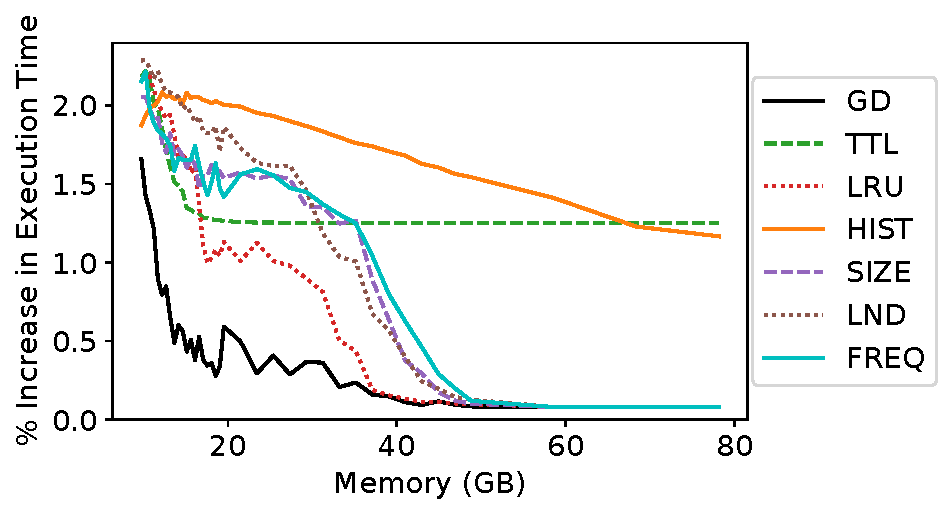
\includegraphics[width=0.4\textwidth]{../graphs/rep-funcs-392/exec_inc_mem-392-legend.pdf}
  \caption{Our caching-based keep-alive policies (such as Greedy-Dual) can reduce the cold-start overhead by more than $3\times$ compared to current (TTL) and state of the art approaches (HIST~\cite{shahrad_serverless_2020}). The results are shown for a representative sample of the Azure function trace comprising of over 100 million function invocations.}
  \label{fig:392-b-trace}
\end{figure}


\subsection{Caching-based Resource Provisioning}
\vspace*{\subsecspace}

The fundamental challenge underlying resource provisioning for FaaS workloads is the performance vs. resource allocation tradeoff. 
Running a workload on large servers/VMs provides more resources for the keep-alive cache, which reduces the cold-starts and improves the application performance.
We develop a \emph{static} provisioning policy that determines the server memory size for a given function workload, that uses hit-ratio curves that are constructed using the notion of reuse-distances. 

To handle highly dynamic function workloads, our system also dynamically scales VMs up or down (vertical auto-scaling). 
Our \emph{dynamic} VM-sizing approach uses hit-ratio curves and a proportional controller, to minimize both the cold-start overhead and the VM size.
Our provisioning policies are also evaluated using the Azure function trace, as illustrated in Figure~\ref{fig:dynamic}, which shows the dynamic server memory adjustment in response to the function workload using our hit-ratio curve and proportional control based method. 

\begin{figure}[t]
    \vspace*{\myfigspace}
  \centering 
  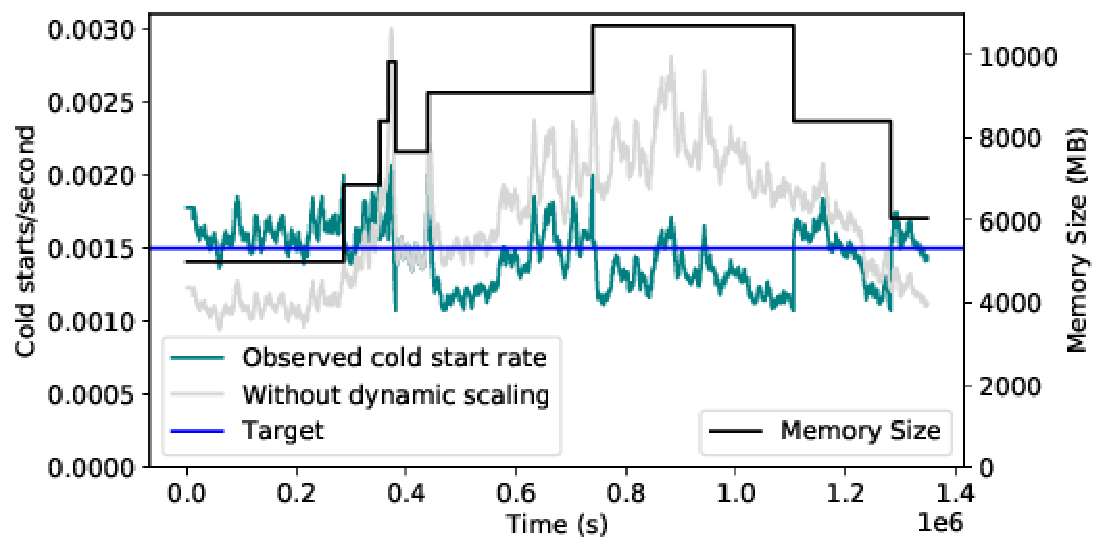
\includegraphics[width=0.4\textwidth]{../graphs/dyn-scale-392-b.pdf}
    \vspace*{\myfigspace}
  \caption{With dynamic cache size adjustment, the cold starts per second are kept within a band, which reduces the average server size by 30\%.}
  \label{fig:dynamic}
  \vspace*{\myfigspace}
\end{figure}



\paragraph{Empirical findings.}
 We implement our caching-based techniques in a popular FaaS platform, OpenWhisk, and empirically evaluate our techniques on real-world FaaS workloads.

\begin{enumerate}
%\item We show the equivalence between caching and function keep-alive, and develop a family of caching-based keep-alive policies for reducing  function cold-start overhead. We use a Greedy-Dual based approach that is designed to work even with the diverse FaaS workloads. 
\item  We conduct extensive trace-driven analysis of the tradeoffs of keep-alive techniques under different workload characteristics based on the Azure FaaS traces~\cite{shahrad_serverless_2020} and popular FaaS applications~\cite{kim_functionbench_2019}. 
    Our experimental results indicate that caching-based keep-alive can reduce cold-start overheads by $3\times$,
  improve application-latency by $6\times$,
  and reduce system load to run $2\times$ more functions.
  \item Our resource provisioning policies use hit-ratio curves to determine the ideal server configuration (such as memory size) required to handle different function workloads. The proportional-control based dynamic vertical-scaling approach can adjust server resources to reduce the cold-start probability, and reduce the average server size by more than $30\%$. 

\end{enumerate}



\section{Why ASPLOS}
\vspace*{\subsecspace}
This paper combines the most cross-cutting area in computer systems, caching, with resource management for Functions as a Service clouds. 
We use caching techniques typically used in storage systems and CDNs. 
Our unique use of caching for keep-alive will interest a broad swathe of the caching experts in all different systems areas.
We also combine serverless computing with virtual machine overcommittment. 

\section{Citation for Most Influential Paper Award}
\vspace*{\subsecspace}

This paper presents a surprising equivalence between Functions as a Service and caching, and lays the groundwork for a new family of principled keep-alive techniques. 
The general, caching-based keep-alive and resource provisioning techniques developed in this paper strengthen the theoretical and practical foundations of serverless computing performance. 


\bibliographystyle{plain}
\bibliography{faas}

\end{document}

%%% Local Variables:
%%% mode: latex
%%% TeX-master: t
%%% End:
